\section{Addition}
\begin{frame}[fragile]
  \frametitle{Addition}
  \framesubtitle{Algorithm}
  \begin{block}{\textit{badd} -- bitwise-optimized addition of big integers}\scriptsize
    \textbf{Input:} \quad Big integer $u$ and $v$ of size $m$ in base $B$\newline
    \textbf{Output:} \,Big integer $w$ of size $m$ in base $B$\newline
\begin{lstlisting}[language=pseudo,escapeinside=!!,basicstyle=\scriptsize]
(ws, cs) = map2 !$\oplus$! us vs
pcs = scan_exc !$\otimes$! 2 cs
w = map2 (!$\lambda$! w c !$\to$! w + (c & 1) ) ws pcs
\end{lstlisting}\phantom{~}\newline
    \textbf{where}\vspace*{-0.5em}
    \begin{align}
  x \oplus y &\coloneq \tup{r}{\mathtt{uint}(r < x)~|~(\mathtt{uint}(r == B-1) \ll 1)},\quad\textbf{where}~r = x + y \\
  x \otimes y &\coloneq (((x~\&~(y \gg 1))~|~y)~\&~1)~|~(x~\&~y~\&~2)
      \end{align}
  \end{block}
\end{frame}

\begin{frame}[fragile]
  \frametitle{Addition}
  \framesubtitle{Implementation 1/2}
  Optimizations boils down to:
  \begin{itemize}
    \item Sequentialize the parallelism in excess.\pause
    \item Segmented scan with flags integrated in the bitwise carry-overflow representation.
    \end{itemize}
  \end{frame}

\begin{frame}[fragile]
  \frametitle{Addition}
  \framesubtitle{Implementation 2/2}
  Implementation revolves around a scan:
  \begin{center}
    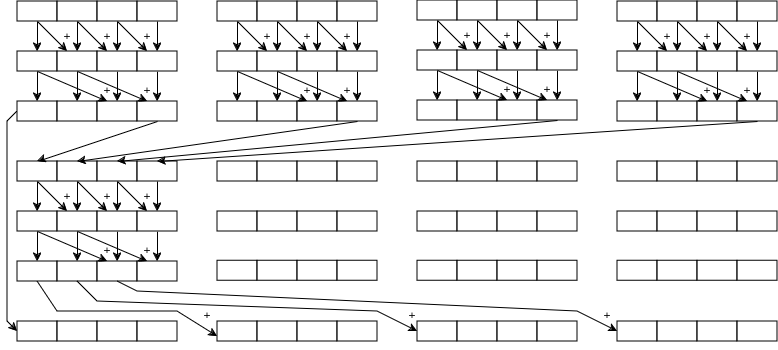
\includegraphics[width=0.875\textwidth]{../thesis/img/warp-level-scan.png}
    \end{center}
\end{frame}

\begin{frame}[fragile]
  \frametitle{Addition}
  \framesubtitle{CUDA 1/3}
  Main addition kernel:
\begin{lstlisting}[language=CPP,gobble=0,basicstyle=\scriptsize,escapeinside=!!,frame=single]
template<class B, uint32_t m, uint32_t q, uint32_t ipb>
__global__ void
baddKer3(typename B::uint_t* as, typename B::uint_t* bs,
                                 typename B::uint_t* rs) {
    using uint_t  = typename B::uint_t;
    using carry_t = typename B::carry_t;
    uint_t ass[q];
    uint_t bss[q];
    cpGlb2Reg<uint_t,m,q,ipb>(as, ass);
    cpGlb2Reg<uint_t,m,q,ipb>(bs, bss);
    __syncthreads();

    uint_t rss[q];
    __shared__ carry_t shmem[m*ipb];
    baddKer3Run<B,m,q,ipb>(ass, bss, rss, shmem);  !\green$\star~\mathit{badd}$!
    cpReg2Glb<uint_t,m,q,ipb>(rss, rs);
}
\end{lstlisting}
\end{frame}

\begin{frame}[fragile]
  \frametitle{Addition}
  \framesubtitle{CUDA 2/3}
  Step 1.
  \begin{lstlisting}[language=CPP,gobble=4,basicstyle=\scriptsize,firstnumber=18,frame=single]
    uint_t css[q];
    carry_t acc = threadIdx.x % (m/q) == 0
        ? SegCarryProp<B>::setFlag(SegCarryProp<B>::identity())
        : SegCarryProp<B>::identity();
    #pragma unroll
    for(int i=0; i<q; i++) {
        rss[i] = ass[i] + bss[i];
        css[i] = ((carry_t) (rss[i] < ass[i]))
                 | (((carry_t) (rss[i] == B::HIGHEST)) << 1);
        acc = SegCarryProp<B>::apply(acc, css[i]);
    }
    shmem[threadIdx.x] = acc;
    __syncthreads();
\end{lstlisting}
\end{frame}

\begin{frame}[fragile]
  \frametitle{Addition}
  \framesubtitle{CUDA 3/3}
  Step 2.
  \begin{lstlisting}[language=CPP,gobble=4,basicstyle=\scriptsize,firstnumber=31,frame=single]
    acc = scanExcBlock< SegCarryProp<B> >(shmem, threadIdx.x);
    acc = threadIdx.x % (m/q) == 0 ? SegCarryProp<B>::identity()
                                   : acc;
\end{lstlisting}
  Step 3.
\begin{lstlisting}[language=CPP,gobble=4,basicstyle=\scriptsize,firstnumber=34,frame=single]
    #pragma unroll
    for(int i=0; i<q; i++) {
        rss[i] += (acc & 1);
        acc = SegCarryProp<B>::apply(acc, css[i]);
    }
\end{lstlisting}
\end{frame}

\begin{frame}[fragile]
  \frametitle{Addition}
  \framesubtitle{Futhark 1/3}
  Main addition function:
\begin{lstlisting}[language=futhark,gobble=0,basicstyle=\scriptsize,escapeinside=!!,frame=single]
def baddV3 [ipb][m]
(us: [ipb*(4*m)]ui) (vs: [ipb*(4*m)]ui) : [ipb*(4*m)]ui =

  let cp2sh (i: i64) = #[unsafe]
    let str = ipb*m
    in ((us[i], us[str + i], us[2*str + i], us[3*str + i])
       ,(vs[i], vs[str + i], vs[2*str + i], vs[3*str + i]))

  let (uss, vss) = map cp2sh (0..<ipb*m) |> unzip
  let (u1s, u2s, u3s, u4s) = unzip4 uss
  let (v1s, v2s, v3s, v4s) = unzip4 vss
  let ush = u1s ++ u2s ++ u3s ++ u4s
  let vsh = v1s ++ v2s ++ v3s ++ v4s

  in baddV3Run ush vsh :> [ipb*(4*m)]ui  !\green$\star~\mathit{badd}$!
\end{lstlisting}
\end{frame}

\begin{frame}[fragile]
  \frametitle{Addition}
  \framesubtitle{Futhark 2/3}
  Step 1.
\begin{lstlisting}[language=futhark,gobble=4,basicstyle=\scriptsize,frame=single,firstnumber=16]
    let (ws, cs, accs) = unzip3 <| imap (0..<ipb*m) (\ i ->
      let i4 = i*4
      let (u1,u2,u3,u4) = (us[i4], us[i4+1], us[i4+2], us[i4+3])
      let (v1,v2,v3,v4) = (vs[i4], vs[i4+1], vs[i4+2], vs[i4+3])
      let (w1,w2,w3,w4) = (u1 + v1, u2 + v2, u3 + v3, u4 + v4)
      let (c1,c2,c3,c4) = (carryAug w1 u1, carryAug w2 u2,
                           carryAug w3 u3, carryAug w4 u4)
      let c1 = (boolToCt (i % m == 0)) << 2 | c1
      let acc = carryProp c1 <| carryProp c2 <| carryProp c3 c4
      in ((w1, w2, w3, w4), (c1, c2, c3, c4), acc))
\end{lstlisting}
  Step 2.
\begin{lstlisting}[language=futhark,gobble=4,basicstyle=\scriptsize,firstnumber=27,frame=single]
    let pcs = scanExc carryPropSeg carryPropE accs
\end{lstlisting}
\end{frame}

\begin{frame}[fragile]
  \frametitle{Addition}
  \framesubtitle{Futhark 3/3}
  Step 3.
\begin{lstlisting}[language=futhark,gobble=4,basicstyle=\scriptsize,firstnumber=28,frame=single]
    let (wi1s, wi2s, wi3s, wi4s) = imap4 ws cs pcs (0..<ipb*m)
      (\ (w1, w2, w3, w4) (c1, c2, c3, _) acc1 i ->
         let acc1 = if i % m == 0 then carryPropE else acc1
         let acc2 = carryProp acc1 c1
         let acc3 = carryProp acc2 c2
         let acc4 = carryProp acc3 c3
         in ((w1 + fromCt (acc1 & 1), i*4),
             (w2 + fromCt (acc2 & 1), i*4+1),
             (w3 + fromCt (acc3 & 1), i*4+2),
             (w4 + fromCt (acc4 & 1), i*4+3))) |> unzip

    let (ws, inds) = unzip <| wi1s ++ wi2s ++ wi3s ++ wi4s
    in scatter (replicate (ipb*(4*m)) 0) inds ws
\end{lstlisting}
\end{frame}

\begin{frame}[fragile]
  \frametitle{Addition}
  \framesubtitle{Evaluation}
  One addition and ten additions of base \texttt{uint64\_t} in GB/s:\newline
  \begin{center}\scriptsize
  \begin{tabular}{|c|c||c|c|c||c|c|c|}\hline
    Bits & I{\tiny nsts} & CGBN1 & CUDA1 & Fut1 & CGBN10 & CUDA10 & Fut10 \\\hline\hline
    $2^{18}$ & $2^{14}$ & 62  & 161 & --   & 25  & 92  & --  \\\hline
    $2^{17}$ & $2^{15}$ & 67  & 163 & --   & 60  & 109 & --  \\\hline
    $2^{16}$ & $2^{16}$ & 19  & 166 & 146 & 73  & 124 & 24 \\\hline
    $2^{15}$ & $2^{17}$ & 19  & 166 & 168 & 45  & 124 & 29 \\\hline
    $2^{14}$ & $2^{18}$ & 84  & 166 & 168 & 97  & 124 & 29 \\\hline
    $2^{13}$ & $2^{19}$ & 164 & 165 & 168 & 162 & 123 & 29 \\\hline
    $2^{12}$ & $2^{20}$ & 165 & 166 & 168 & 164 & 123 & 29 \\\hline
    $2^{11}$ & $2^{21}$ & 164 & 166 & 168 & 161 & 124 & 29 \\\hline
    $2^{10}$ & $2^{22}$ & 156 & 166 & 168 & 152 & 124 & 29 \\\hline
    $2^{9}$  & $2^{23}$ & 118 & 167 & 168 & 113 & 124 & 29 \\\hline
  \end{tabular}
  \end{center}
\end{frame}

%%% Local Variables:
%%% mode: LaTeX
%%% TeX-master: "main"
%%% End:
